%                                             -*- coding: utf-8 -*-
% Mindenkinek csak javasolni tudjuk, hogy latex-et használjon.
% Szakdolgozatnál vagy diplománál már egyértelműen kijönnek az
% előnyei a Worddel szemben.  Ennek ellenére ez a sablon messze nem
% tökéletes.  Ha valamit javítanál benne, kérlek, küld vissza, hogy
% hallgatótársaid is profitáljanak belőle.  Köszönöm.

% További nehézséget okoz, hogy a népszerű latex disztribúciók nem
% tartalmazzák a legújabb változatát a magyar.ldf-nek.  A szükséges
% fájlokat a sablon mellé bemásoltuk, de le is tölthetőek innen:
% http://www.math.bme.hu/latex/
%
%
%
\documentclass[a4paper,oneside]{article}
\usepackage[margin=3cm]{geometry}
% =================================================================
% Magyar nyelvi támogatás
%------------------------
% ###################
% Nyelvváltó parancsok:
%\selectlanguage{english}
%\selectlanguage{magyar}
% rövid angol beszúrás:  \foreignlanguage{english}{some english text}
% határozott névelők generálása ``magyar'' babel-el:
% argumentum+megfelelő határozott nevelő: \az{},\Az{}
% csak a megfelelő határozott nevelő: \az*{}, \Az*{}
% címkék: \aref{}, \aref*{}, képletekhez \aref()
%        \Aref{}, \Aref*{}, képletekhez \Aref()
% oldalak: \apageref{}, \apageref*{}
%        \Apageref{}, \Apageref*{}
% idézetek: \acite, \acite*, \Acite, \Acite*
% ###################
\usepackage[english,magyar]{babel} %vegyes nyelvi támogatás a
% magyar helyesírás ellenőrzéshez (ispell) és elválasztáshoz
\selectlanguage{magyar}

%=================================================================
% direkt ékezetes karakter beírás támogatás
%-------------------------------------------
\usepackage[T1]{fontenc}
\usepackage[utf8]{inputenc}
\usepackage{multirow} 
%================================================================
% Undorító dolog bitmappelt (Type III) betűtípust nézni a PDF-ben
% képernyőn. Az alapértelmezett Computer Modern font LaTex-ben
% bitmappelt, ezért használjunk Times fontot:
\usepackage{times}

%================================================================
% ha ábrát akarunk beemelni, akkor használjuk a graphicx/graphics
% csomagot és az \includegraphics[width=<width>]{abra.pdf} parancsot
\usepackage{graphicx} %for graphics
%kepek helye a gyokerhez(ehhez a file-hoz kepest) kepest
\graphicspath{{./figs/}}

%================================================================
% Kötelezően használjuk a hyperref csomagot, mert ezzel többek között 
%  kultúrált hyperlinkelt PDF-et lehet csinálni az alábbi
%  variációkban, különféle hyperref backend-ekkel:
%  pdflatex,dvipdfm,ps2pdf
% tapsztalataim szerint a MikTeX (Win32) a 'dvipdfm' konverzióval
% optimális  míg a teTeX (Linux/Solaris) jobb szereti a 'dvips' módszert
%------------------------------------
% pontosan egyet kommentezzünk be!!!!!!!
% értelemszerűen backend függően generáljunk dvi-ból PDF-et!!!
%------------------------------------
% A hyperref csomag az utolsó beolvasott csomag legyen, kivéve néhány
% problémás csomagot, pl. algorithm
%-----------
% ########################### FONTOS ###########################
% A hyperref hibásan működik a babel csomag 'magyar.ldf' fájljának
% 1.5-ös verziójánál korábbi változatával. 2004. februárjában a MikTeX
% és teTex disztribúciók még csak a v.1.4 verziót tartalmazták! A fájl
% aktuális verziója a BME Matematikai intézet LaTeX honlapjáról
% elérhető: http://www.math.bme.hu/latex/ 
% A lusták kedvéért a jelen sablon mellé is mellékelem:
% magyarlatex_0.01-2.tar.gz 
% ########################### FONTOS ###########################
%-----------
\usepackage[colorlinks=true]{hyperref}

%%%%%%%%%%%%%%%%%%%%%%%%%%%%%%%%%%%%%%%%%%%%%%%%%%%%%%%%%%%%%%%%%%%
% Itt kezdődik maga a dokumentum
%%%%%%%%%%%%%%%%%%%%%%%%%%%%%%%%%%%%%%%%%%%%%%%%%%%%%%%%%%%%%%%%%%
\begin{document}
%%%%%%%%%%%%%%%%%%%%%%%%%%%%%%%%%%%%%%%%%%%%%%%%%%%%%%%%%%%%%%%%%%%
% Ezt ne piszkáld!!!!
%%%%%%%%%%%%%%%%%%%%%%%%%%%%%%%%%%%%%%%%%%%%%%%%%%%%%%%%%%%%%%%%%%%
\pagestyle{myheadings} % legyen fejléc 

\newcommand{\onlabcim}{
  \begin{center}
    \huge{\textbf{Önálló laboratórium beszámoló}}

    \small{Távközlési és Médiainformatikai Tanszék}
  \end{center}
} 

% Argumentumok: #1=Név, #2=Neptunkód, #3=szakirány, #4=email, #5 konzulens-1, #6 konzulens-1-email, #7 konzulens-2, #8 konzulens-2-email
\newcommand{\onlabszerzo}[8]{

\begin{center}
  \begin{tabular}{ r l }
  készítette: & \textbf{#1}  \\
              & \href{mailto:#4}{\textbf{#4}}  \\
  neptun-kód: & \textbf{\texttt{#2}}  \\
  ágazat:     & \textbf{#3}  \\
  konzulens: & \textbf{#5}  \\
             & \href{mailto:#6}{\textbf{#6}} \\
  konzulens: & \textbf{#7}  \\
             & \href{mailto:#8}{\textbf{#8}}  \\
  
  \end{tabular}
\end{center}

}

% % Argumentumok: #1=Név, #2=email
% \newcommand{\konzulens}[2]{
%   \noindent\textbf{Konzulens:} #1 
%   \newline\emph{Email cím:}\/ \href{mailto:#2}{#2}
%   \newline
% 
% }

% Argumentumok: #1=Tanév (xxxx/xx alakban, #2=félév (pont nélkül)
\newcommand{\tanevfelev}[2]{
  \large\noindent\textbf{Tanév:} #1. tanév, #2. félév
  \newline
}

% Argumentumok: #1=téma címe 
\newcommand{\feladatcim}[1]{
  \large\noindent\textbf{Téma címe: #1}
  \bigskip
}

% Argumentumok: #1=téma részletei 
\newcommand{\feladatmaga}[1]{
\large\noindent\textbf{Feladat:} 
  \newline
 #1
 \newline
 \smallskip
}

% A fejezetek közé beágyazott irod.jegyzék
\def\thebibliography#1{\renewcommand{%
\baselinestretch}{1}\subsection{A tanulm\'anyozott irodalom jegyz\'eke}\list
 {\small [\arabic{enumi}]}{\settowidth\labelwidth{[#1]}\leftmargin\labelwidth
 \advance\leftmargin\labelsep
 \usecounter{enumi}}
 \def\newblock{\small \hskip .11em plus .33em minus .07em}
 \sloppy\clubpenalty4000\widowpenalty4000
 \sfcode`\.=1000\relax}
\let\endthebibliography=\endlist%


%%% Local Variables: 
%%% mode: latex
%%% TeX-master: "template"
%%% End: 
 % Ez kell!!!
\markright{Beszámoló Péter (BPOX43)} % egyoldalas fejléc!!!
%--------------------------------------------------------------------
% fedlap
%--------------------------------------------------------------------
\begin{titlepage}
%bme logo 
 \begin{figure}[h]
    \centering
      
\includegraphics[width=12cm]{bme_logo}
  \label{fig:bme_logo}
  \end{figure}
  \thispagestyle{empty}
  %cím generálás
  \onlabcim

% \begin{center}
%   \begin{tabular}{ p{3cm} p{5cm} }
%   
%   Készítette: & Beszámoló Péter  \\
%   Neptun-kód: & BPOX43  \\
%   Ágazat: & Médiainformatika  \\
%   E-mail cím: & b.peter@onlab.hu  \\
%   Konzulens: & Dr. Péhádes István  \\
%   E-mail cím: & pehades@tmit.bme.hu  \\
%   Konzulens: & Doktor Andusz  \\
%   E-mail cím: & doktora@tmit.bme.hu  \\
%   
%   \end{tabular}
% \end{center}

 
  %\szerzo argumentumok: #1=Név, #2=Neptunkód, #3=szakirány, #4=email,#5 konzulens-1, #6 konzulens-1-email, #7 konzulens-2, #8 konzulens-2-email
  \onlabszerzo{Beszámoló Péter}{BPOX43}{Ilyen-olyan szak}{user@example.com}{Dr. Péhádes István}{pehades@tmit.bme.hu}{Doktor Andusz}{doktora@tmit.bme.hu}
 
 
%\feladatcim argumentuma a feladat rövid, 1 soros címe
  \feladatcim{Írásbeli beszámoló készítése az Önálló laboratórium
    tárgyhoz} 

  <A címnek nem kell megegyeznie az eredeti téma címével,
  fontosabb hogy tényleges feladatra utaljon.>


  %\feladatmaga argumentuma a feladat 1-2 bekezdésnyi ismertetése
  \feladatmaga{<Ezen a helyen a hallgató adott félévre vonatkozó
    feladatának a leírását várjuk.  A hallgató ezt idemásolhatja a
    feladatkiírásból, esetleg a munkatervéből, de megadhatja saját
    szavaival is.  Ha a munkatervéből másolja ide, akkor folyószöveggé
    kell szerkeszteni az időrendi bontást. A feladat leírása ne
    csússzon át a 2. oldalra és ezáltal a tanév sem. A feladatleírás
    legyen konkrét, definiálja, hogy mit várunk el a félév végére és
    ne legyen felsorolás-szerű.>}

 
  %\tanevfelev argumentumok:
  % #1=Tanév (xxxx/xx alakban), #2=félév (pont nélkül!)
  
  \tanevfelev{2016/17}{I}
 
\end{titlepage} 

%==================================================================
\section{A laboratóriumi munka környezetének ismertetése,
     a munka előzményei és kiindulási állapota}
\label{sec:kornyezet}
% A munka  előzményei és kiindulási állapota
% \newpage
\subsection{Bevezető}
\label{sec:bevezeto}

<Mit kell tudni a feladatról, esetleges elméleti bevezető (nagyon
értelemszerű dolgokat ne definiáljunk, de jó, ha egy kicsit
kontextusba kerül a témakör, miért fontos ez nekünk, mi volt eddig,
milyen megoldások jöhetnek szóba és miért emellett döntöttünk, milyen
kari nagyobb projektbe kapcsolódik ez), stb. Terjedelem max. 50\%
beszámolónak.>

Ennek a résznek az a szerepe, hogy az olvasó számára megmutassa az
elvégzett munka tágabb környezetét. Ez a rész lehet megegyező tartalmú
más, ugyanazon a témán dolgozó hallgatókéval, de akkor mindenképpen
tüntessük fel, hogy kivel dolgoztatok együtt, és hogy pontosan, hogy
osztottátok meg a munkát.

\subsection{Elméleti összefoglaló}

Amikor a tágabb tudományos vagy műszaki környezetről beszélünk, akkor
azt értjük alatta, hogy ,,művelt laikus'' -- alapesetben ennek
tekinthető a tárgyfelelős -- megtalálja azokat a kapcsolódási
pontokat, amelyek segítségével az ő ismereteihez a beszámolóban
tárgyalt témakör és az elvégzett munka csatlakoztatható.  Ez
mindenképpen, szükséges, hiszen enélkül az olvasónak előzetes
tájékozódást kellene végeznie a szűkebb szakterületen, hogy az
elvégzett munka jellegét, súlyát, nehézségét meg tudja ítélni.

Természetesen a terjedelmi korlátok miatt nem lehet teljes mértékben
bemutatni az adott szűkebb szakterületet, ezért meg kell adni az
érdeklődő olvasónak a lehetőséget a további tájékozódásra.  Részben
erre szolgálnak a hivatkozások\footnote{A másik nagyon fontos céljuk
  az állítások alátámasztása.  A lábjegyzetek használatát egyébként
  nem érdemes túlzásba vinni, mert állandóan megtörik az olvasás
  folyamatát (lásd például \cite{esterhazy}).  Akkor kell használni,
  amikor a lábjegyzetben közlendő információ érdekes lehet, de nem
  tartozik közvetlenül a tárgyhoz.  Mindenképpen kerülendő az irodalmi
  hivatkozások lábjegyzetben való megadása.}, lábjegyzetek.

Nagyon fontos, hogy abban az esetben, amikor a hallgató féléves
munkájának egy része vagy egésze az, hogy tanul, hogy maga is
ismerkedik azzal a szakterülettel, amelyen dolgozni fog, akkor az
tudatosan törekedjen arra, hogy az Elméleti összefoglaló és az
Elvégzett munka ismertetése szétválasztható legyen.  Az előbbinek a
szakterület alapvető, általános ismereteit kell tartalmaznia,
amelyekről a ,,művelt laikusnak'' részleges ismeretei lehetnek.  Míg
az elvégzett munka leírásába azoknak a specifikus ismereteknek a
bemutatása kerülhet, amelyek a később elvégzett vagy elvégzendő
feladatokat konkrétan megalapozzák.

További tanulmányozásra ajánljuk Eco professzor művét~\cite{eco}.

A hivatkozások kezelésénél fontos, hogy mindig a mondat részeként
tekintsünk rá, és ha szükséges, akár többször is hivatkozzunk meg egy
forrást, de az első előfordulásakor mindenképpen.  Ugyanez érvényes a
rövidítésekre: minden rövidítést a legelső előforduláskor magyarázni
kell, később viszont használhatók a rövidített formák is.  Például: a
Tiger Tree Hash (TTH) a hashelés egy speciális formája.

\subsection{A munka állapota, készültségi foka a félév elején}
\label{sec:munka-allap-kesz}

Ebben a részben lehet megadni a korábbi félévekben elvégzett munkát
is.  Így világosan elkülöníthető az aktuális félévtől.  Nem kell
hosszasan írni, de ne legyen felsorolás sem.  Egy bekezdésben kellene
itt leírni, hogy foglalkoztál-e már ezzel a témával, a tanszéken
dolgozott-e már valaki rajta.  Írd le azt is, hogy mit kaptál kézhez
hozzá segítségként.

\newpage
%==================================================================
\section{Az elvégzett munka és az eredmények ismertetése}
\label{sec:az-elvegzett-munka}


\subsection{A munkám ismertetése logikus fejezetekre tagoltan}
\label{sec:a-munkam-ismert}
<Én magam (nem a társam) a félév során következőket olvastam el /
programoztam / készítettem el / teszteltem / dokumentáltam / néztem át
/ tanultam meg, stb.  Tételes leírása és felsorolása mindannak, ami a
félév során történt, alátámasztandó azon állításom a
konzulens/tárgyfelelős felé, hogy összességében mindent beleértve
tényleg dolgoztam a TVSZ szerint kreditenként 30 órát, azaz a heti 2
kontakt órás tárgy esetében min. $2,5*30 = 75$ munkaórát, illetve a
heti 6 kontakt órás tárgy esetében min. $8*30 = 240$ munkaórát\dots>

Ebben a részben a hallgató az általa elvégzett munkát mutatja
be. Hangsúlyosan a saját munka bemutatása a cél, hiszen a hallgató
ezzel igazolja a témavezető és a tárgyfelelős irányába, hogy --
folyamatosan fejlődve és egyre több és jobb munkát végezve -- a
szakdolgozatát/diplomadolgozatát képes lesz megírni.  A beszámoló nem
munkanapló, nem arra vagyunk kíváncsiak, hogy mit mikor csinált a
hallgató és mennyi időt töltött vele, hanem egy eredmény-centrikus
beszámolót szeretnénk olvasni.  De itt is fontos tudni, hogy
megosztott feladat esetén ki-mit csinált, mekkora részt vállalt.

Az egész beszámoló elkészítésénél törekedni kell a magyar nyelv
szabályainak követésére és a műszaki dokumentáció/tudományos közlemény
írásával kapcsolatosan kialakult közmegegyezés szerinti formai
követelmények betartására.  (Tehát nem kell többes számként hivatkozni
saját magunkra, kerülni kell a furcsa megfogalmazást, passzív és egyéb
kifacsart mondatszerkezeteket.  Az egy szót határozatlan névelőként
történő használatakor ne írjuk ki számként.)


A beszámoló természetesen nem csak szöveget tartalmazhat, hanem
képleteket, táblázatokat, ábrákat és még sok minden mást.  Ezek
kapcsán az alábbi elvek irányadók:
\begin{itemize}
\item Az ábráknak, képeknek és táblázatoknak mindig van számuk és
  címük. (A cím nem ennyi: ,,1. ábra'', hanem azt írd le, ami látható
  rajta.)

\item Az ábrákra, a képekre és a táblázatokra a szövegben hivatkozni
  kell, és a szövegben elemezni kell azokat. Például
  \aref{fig:fig1}.~ábrán látszik, hogy a vizsgált félévben még két
  napos csúszással is lehetett jeles érdemjegyet szerezni a tárgyból,
  de a pontosság még nem garancia a jó jegyre: öten nem kaptak jelest,
  noha nem késtek a leadással.

\item Az ábrák, képek és táblázatok mérete a szükségesnek megfelelő
  legyen: elég nagy ahhoz, hogy kinyomtatva is olvasható és
  értelmezhető legyen, de nem nagyobb annál, mint amit szerepe
  indokol.

\item A grafikonoknak a tengelyeken legyenek feliratai és ha releváns,
  a mértékegység is.

\item A képletek esetében nem minden képletre történik hivatkozás, de
  ahol igen, ott a képletet a műszaki irodalomban jellemző módon a sor
  végére tett kerek zárójelben lévő számmal jelöljük meg.  A
  képleteket ne képként illeszd be a szövegbe.

\item Kódrészleteket, ha nem relevánsak, ne illeszd be képként, főleg
  ne rossz minőségben. Nyugodtan teheted függelékbe és hivatkozd be a
  szövegben, mint a képeket, például: Az 1.~számú függelékben
  található az adatbeolvasó kód, melyet C++ nyelven készítettem el.
\end{itemize}

Az írásbeli beszámolót a témavezető és a tárgyfelelős is értékeli. A
tárgyfelelősi értékelés szempontjai az alábbiak:
\begin{enumerate}
\item Megfelel-e az elvégzett munka a félév elején kiadott feladatnak?
\item Megfele-e a beszámoló a formai követelményeknek? Ezen belül:
  \begin{itemize}
  \item a. Megfelelő-e az elméleti bevezető és az irodalomjegyzék?
  \item b. Egyértelmű-e, hogy mi volt a hallgató saját munkája?
  \item c. Megfelelő-e a dokumentum technikai színvonala?
  \end{itemize}

\end{enumerate}
Ezen kívül a tárgyfelelős veszi figyelembe az értékelés során
kialakult félévi jegyre vonatkoztatva az ún. ,,hanyagsági faktor''
értékét, amelyet (\ref{eq:1}) szerint állapítunk meg:

\begin{equation}
    F_{hany} = 1 - a - b
  \label{eq:1}
\end{equation}


\begin{figure}[tbh]
  \centering
  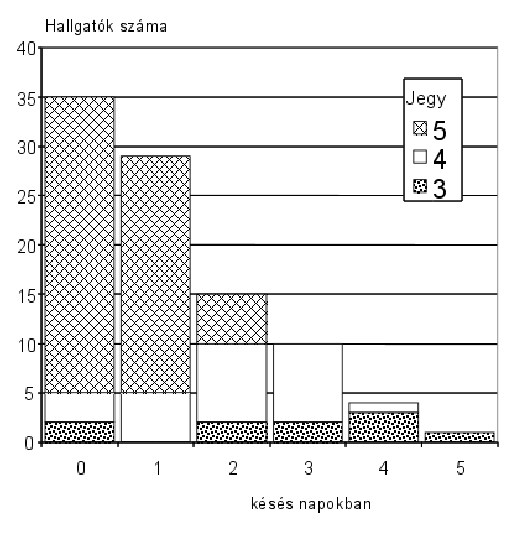
\includegraphics[]{fig1.eps}
  \caption{Hallgatók érdemjegyeinek eloszlása az írásbeli beszámoló késése függvényében}
  \label{fig:fig1}
\end{figure}

Az (\ref{eq:1})-ben szereplő a szám a munkaterv beadásában történt
késedelemre, míg a b szám az írásbeli beszámoló beadásában történt
késedelemre vonatkozik.  Utóbbi értékeiről
\aref{tab:hanyagsagi}.~táblázat tájékoztat.

\begin{table}
  \centering
    \begin{tabular}{|l|c|}
      \hline
      Az írásbeli beszámoló beadásának napja     & A ,,b'' faktor értéke \\
      a szóbeli beszámolóhoz képest (munkanapban) & ~ \\ \hline          
      -4.~munkanap & $0.04$ \\ \hline 
      -3.~munkanap & $0.09$ \\ \hline 
      -2.~munkanap & $0.20$ \\ \hline 
      -1.~munkanap & $0.30$ \\ \hline
      \end{tabular}
    \caption{Az írásbeli beszámoló késedelmes beadásával kapcsolatos hanyagsági faktor értéke}
  \label{tab:hanyagsagi}
\end{table}

A beszámoló értékeléséről részletesebben írunk \cite{web}-ban.

A beszámolóban bizonyára szerepelni fognak rövidítések. Ezeket a
rövidítéseket, betűszavakat néhány, az infokommunikáció területén
nagyon ismert és gyakran használt kifejezéstől (például IP, TCP, GPRS,
UMTS) eltekintve ki kell fejteni logikusan az első használat
alkalmával (például így: ,,A GPS (Generalized Processor Sharing) egy
ideális folyadékmodellen alapuló csomagütemező eljárás.'').

A beszámoló készítése során előfordulhat, hogy a hallgató úgy érzi,
hogy alfejezetekkel tagolva jobban olvasható és érthető lenne a
beszámoló.  Ennek akadálya nincs, de érdemes arra figyelni, hogy a
túlzott tagolás sem tesz jót egy írásműnek, illetve hogy a címsorokban
a rövidítések és a hivatkozások használata tilos.  Tartalomjegyzéket
készíteni nem szükséges a beszámolóhoz, de nem is tilos, kivéve azt az
esete, amikor nyilvánvalóan terjedelemnövelési célokat szolgál.

A beszámoló terjedelme tárgyanként változhat.  Általános szabály, hogy
1 hüvelyknél nagyobb margókat ne használjunk.  A szöveg legyen
egyszeres sortávú, sorkizárt és 12 pontos betűméretű.  A bekezdések
kezdődjenek behúzással a minta szerint.

\subsection{Összefoglalás}
\label{sec:osszefoglalas}

A félévi munka során elért új eredmények ismételt, vázlatos, tömör
Ebben a részben az adott félévre vonatkozó, az \emph{Önálló
  laboratórium tárgy keretében elvégzett munka során} elért
\textbf{új} eredmények ismételt, vázlatos, \textbf{tömör}
összefoglalását várjuk, lehetőleg nem felsorolásként.  Itt még egyszer
ki lehet térni a leglényegesebb eredményekre, valamint a félév során
felmerülő nehézségekre, de meg lehet említeni a továbbfejlesztési
irányokat, lehetőségeket is.

Ezt a részt tagolható a következő pontok megválaszolásával:
\begin{itemize}
\item Mi volt az \textbf{aktuális kérdés}, probléma, amivel a félév
  során foglalkoztál?
\item Mi a dolgozat \textbf{célja}, miért érdekes egyáltalán ezzel a
  problémával foglalkozni?
\item Milyen \textbf{módszereket} használtál a probléma megoldása
  érdekében?
\item Mik a legfontosabb \textbf{eredmények}?
\item Milyen \textbf{következtetéseket} lehet levonni?

\end{itemize}

Ha valaki elolvassa ezt a részt, képet kell kapnia az egész
dolgozatról.  Ne legyen az absztrakt szó szerinti ismétlése.

Fontos, hogy az itt megadott sablontól el lehet térni, használata nem
kötelező, csak segítséget jelenthet, viszont a fedőlap lehetőleg
maradjon ugyanez és tartalmilag egyezzen meg a sablon irányelveivel. A
beszámoló felépítésében nem érdemes eltérni a \emph{Bevezető --
  Féléves munka és eredmények bemutatása -- Összefoglaló} hármastól.

\newpage
 
%==================================================================
\section{Irodalom, és csatlakozó dokumentumok jegyzéke}
\label{sec:irod-es-csatl}

\begin{thebibliography}{9}
\label{sec:tanulm-irod-jegyz}

\bibitem{eco} Umberto Eco, \emph{Hogyan írjunk szakdolgozatot?},
  Kairosz Kiadó, 2000, ISBN: 9639137537.

\bibitem{esterhazy} Esterházy Péter, \emph{Termelési-regény (Kisssregény),}
  Magvető Könyvkiadó, 2004, ISBN: 9631423948.

\bibitem{web} \emph{Tájékoztató a Műszaki Informatika Szak önálló
    laboratórium tantárgyainak 2008/9. tanév I. félévi lezárásáról a
    BME TMIT-en (VITMA367, VITMA380, VITT4353, VITT4330),}
  \url{http://inflab.tmit.bme.hu/08o/lezar.shtml}, szerk.: Németh Felicián,
  2008. november 5.

\bibitem{wikipedia} Wikipedia contributors, \emph{Wikipedia:Academic
    use}, Wikipedia, The Free Encyclopedia, 2011 Nov 11.  Available
  from: \\ \url{http://en.wikipedia.org/w/index.php?title=Wikipedia:Academic\_use\&oldid=460041928}

\end{thebibliography}

Itt jegyezném meg, hogy a tanulmányozott irodalmat hivatkozni kell a
szövegben.  Szükség esetén többször is.  Az irodalomjegyzék célja
(lásd \aref{sec:tanulm-irod-jegyz} fejezetet) ugyanis
kettős\footnote{Akárcsak ennek a fejezet hivatkozásnak, ami a
  \texttt{$\backslash$aref babel} parancsot demonstrálja}:
\begin{enumerate}
\item Az olvasó tájékoztatása, hogy a dokumentumban ki nem fejtett
  dolgoknak, a tudottnak vélt ismereteknek hol lehet bővebben
  utánanézni, így ott kell meghivatkozni az irodalmat~\cite{eco,
    esterhazy}, ahová az irodalom kapcsolódik.
\item Megmutatni a tárgyfelelosnek/konzulesnek az elolvasott irodalom
  mennyiségét
\end{enumerate}

Javasoljuk, hogy a hallgatók tanulmányozzák, hogyan néznek ki a
hivatkozások a villamosmérnöki/informatikai szakma vezető szakmai
folyóirataiban megjelenő cikkekben.  Ebben a témavezető is biztosan
tud segíteni.  A hivatkozás teljességére és egyértelműségére tessék
ügyelni.  Például, ha egy könyvnek több, eltérő kiadása is van, akkor
azt is meg kell jelölni, hogy melyik kiadásra hivatkozunk.  A webes
hivatkozások problémásak szoktak lenni, de manapság egyre több az
olyan dokumentum, ami csak weben lelhető fel, ezért használatuk nem
zárható ki. Itt is törekedni kell azonban a pontosságra és a
visszakereshetőségre. A weben található dokumentumoknak is van címe,
szerzője, illetve érdemes megadni a letöltés/olvasás időpontját is,
hiszen ezek a dokumentumok idővel megváltozhatnak.

A wikipédiás hivatkozások használata nem javasolt, mert a wikipedia
másodlagos forrás.  Tájékozodjuk a wikipédián, de aztán olvassuk el az
adott oldalhoz megadott hivatkozásokat is.  A wikipedián külön szócikk
foglalkozik azzal, hogy miért nem szerencsés tudományos munkákban a
wikipédiára hivatkozni \cite{wikipedia}.

Nem publikus dokumentumok hivatkozása nem javasolt és csak kivételes
helyzetben elfogadható!

%==================================================================
\subsection{A csatlakozó dokumentumok jegyzéke}
\label{sec:csat-irod}

<A munka ezen beszámolóba be nem fért eredményeinek (például a forrás
fájlok, mindenképpen csatolni akart forráskód részlet, felhasználói
leírások, programozói leírások (API), stb.) megnevezése,
fellelhetőségi helyének pontos definíciója, mely alapján a az
erőforrás előkereshető -- értelemszerűen nem nyilvános dokumentumok
hivatkozása nem elfogadható.>

\end{document} 

%%% Local Variables: 
%%% mode: latex 
%%% TeX-master: t 
%%% End:

